\subsection{Authorization}

Das Authorization Pattern beschreibt auf einfache Art und Weise die Zugriffsberechtigungen eines Subjekts auf ein bestimmtes Objekt. Es spezifiziert zudem die Art des erlaubten Zugriffes (Lesend, schreibend etc.)

\subsection*{Kontext}
Jegliche Umgebungen in denen der Zugriff auf enthaltene Objekte kontrolliert werden muss.

\subsection*{Problem}
In einer kontrollierten Umgebung muss sichergestellt werden, dass nur berechtigte Subjekte auf entsprechende Objekte zugreifen können. Es stellt sich also die Herausforderung, diese Information losgelöst von den eigentlichen Objekte abzulegen. Dabei soll aber eine gewisse Flexibilität bei der Definition von Berechtigungen, Objekten und Subjekten erhalten bleiben.

Des weiteren sollen diese Informationen so einfach wie möglich im Nachhinein änderbar sein.

\subsection*{Lösung}
Strukturell fällt die Lösung zum Authorization Pattern relativ simpel aus:

\begin{figure}[H]
	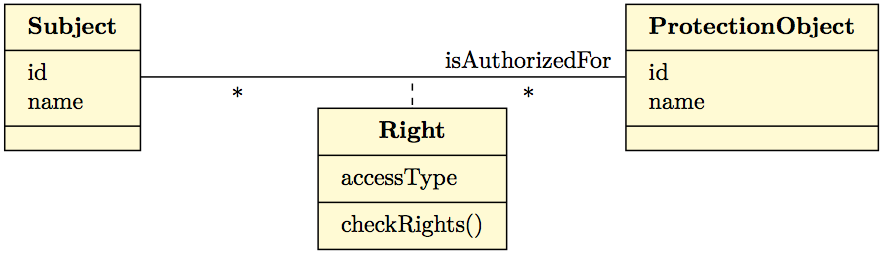
\includegraphics[width=\textwidth]{content/security/accesscontrolmodels/images/authorization.png}
\caption{Authorization Klassendiagramm}
\end{figure}

\begin{itemize}
	\item Subject beschreibt jegliche Aspekte des zu berechtigenden Subjekts
	\item Das ProtectionObject ist das zu schützende Objekte
	\item Right enthält alle Informationen, wie Subject auf ProtectioObject zugriefen darf/kann
\end{itemize}

\subsection*{Erweiterungen}
Die vorgestellte Struktur kann um komplexere Aspekte erweitert werden. So kann bspw. mittels einem ''Copy''-Flag eine Stellvertretung eines Subjektes durch ein anderes ermöglicht werden.
Weiter ist die Verwendung eines Prädikats denkbar, welches eine Regel mit zusätzlicher ''Intelligenz'' austatten kann (-> ''Darf nur zugreifen wenn Zeit innerhalb Arbeitszeit'')

Diese Anpassungen können direkt auf dem Rights-Objekt modelliert werden.

\subsection*{Vor- \& Nachteile}
\begin{itemize}
	\item Durch seine Offen- und Allgemeinheit kann dieses Pattern auf jegliche Umgebung appliziert werden (Filesysteme, Organistaitonsstrukturen, Zugangskontrollen etc.)
	\item In der beschriebenen Form sind administrative Aufgaben (Änderung der Zugriffsrechte) nicht gesondert definiert. Für bessere Sicherheit ist dies jedoch von Vorteil
	\item Für viele Subjekte/Objekte müssen entsprechend viele Berechtigungsregeln erfasst und auch verwaltet werden
	\item Viele Regeln machen die Verwaltung für einen Administrator zu einer heiklen Aufgabe (Verkettung von Berechtigungen etc.)
\end{itemize}

\subsection*{Beispielanwendungen}
\begin{itemize}
	\item Dateisysteme
	\item Firewalls greifen teilweise auf dieses Pattern zurück, um Regeln für den analysierten Traffic zu modellieren
\end{itemize}

\subsection*{Mögliche Prüfungsfragen}
\begin{itemize}
	\item \emph{Macht es Sinn, auch verbietende Regeln zu erfassen?}\\
	Möglich wäre dies bestimmt, im Normalfall verkompliziert dies jedoch das Sicherheitskonzept auf allen Ebenen: Die Administration wird undurchsichtiger, die Überprüfung/Durchsetzung der Regeln wird komplexer und es besteht die Möglichkeit, dass sich ein Subjekt komplett ``ausschliessen'' kann. (vgl. Windows Filesystem)
\end{itemize}